 
\chapquote{``Design is choosing how you will fail."}{Ron Fein}

\problem Showcase \textit{class inheritance} in \textit{Java}, by designing a hierarchy of geometric shapes.

\solution Here, we use an interface \texttt{Shape} as the superclass of the interfaces \texttt{Shape2D} and \texttt{Shape3D}, 
each of which has subclasses sharing common behaviour. For example, all $2D$ shapes have computable areas and perimeters, while
all $3D$ shapes have computable volumes and surface areas. This structure illustrates \textit{multilevel inheritance}.

All these shapes can be \textit{scaled}, i.e., their dimensions can be changed by some factor. This behaviour is defined by 
the interface \texttt{Scalable}, which the above classes all implement. This structure illustrates \textit{multiple inheritance}.
The class \texttt{LineSegment} is also \texttt{Scalable}, despite not being a \texttt{Shape}.

\vspace{10mm}

\tikzstyle{vertex}=[draw]
\tikzstyle{edge}=[draw, -latex, >=stealth, line width=0.2mm]

\begin{figure}[htpb]
\begin{center}
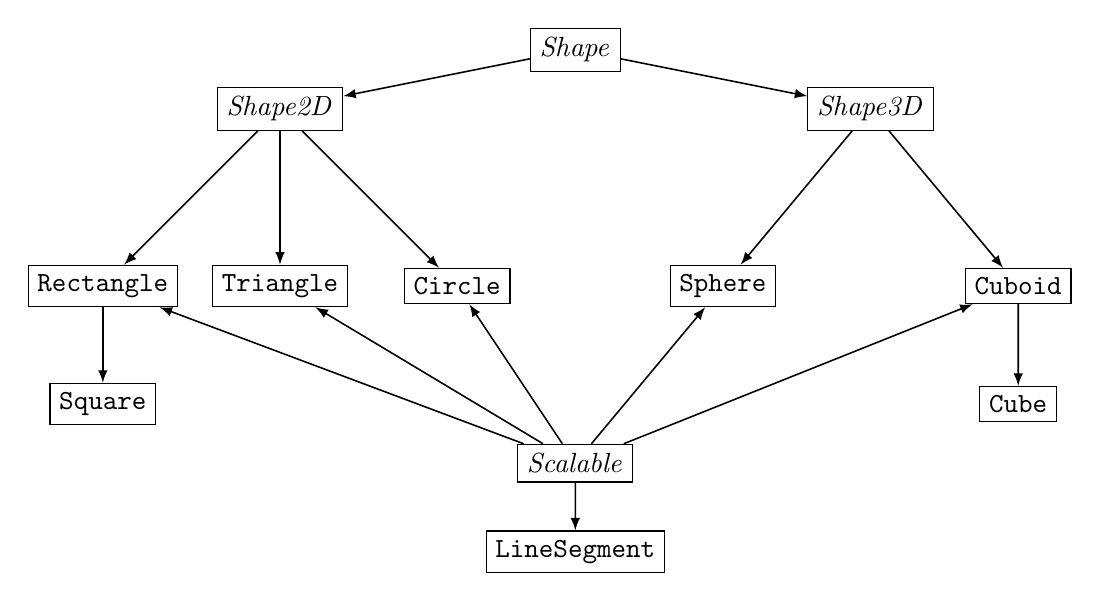
\begin{tikzpicture}[scale=0.75, auto]
	\foreach \pos/\name in {{(6,4)/Circle}, {(3,4)/Triangle}, {(0,4)/Rectangle}, {(0,2)/Square},
				{(10.5,4)/Sphere}, {(15.5,4)/Cuboid}, {(15.5,2)}/Cube, {(8,-0.5)/LineSegment}}
		\node[vertex] (\name) at \pos {\texttt{\name}};
	\foreach \pos/\name in {{(8,8)/Shape}, {(3,7)/Shape2D}, {(13,7)/Shape3D}, {(8,1)/Scalable}}
		\node[vertex] (\name) at \pos {\textit{\name}};
	\foreach \source/\dest in {Shape/Shape2D, Shape/Shape3D, Shape2D/Circle, Shape2D/Triangle,
				   Shape2D/Rectangle, Rectangle/Square, Shape3D/Sphere, Shape3D/Cuboid, Cuboid/Cube,
				   Scalable/LineSegment, Scalable/Circle, Scalable/Rectangle, Scalable/Triangle,
				   Scalable/Sphere, Scalable/Cuboid}
		\path[edge] (\source) -> (\dest);
\end{tikzpicture}
\end{center}
\label{fig:shape_tree}
\end{figure}

\vspace{10mm}

Following is a general implementation of a shape `\texttt{MyShape}', which has a computable property `\texttt{myProperty}' and
is \texttt{Scalable}.

\algorithm
\texttt{MyShape (parameters... :Number)}
\begin{enumerate}
	\item Copy each \texttt{parameter} as an immutable constant into the object data.
	\item \textbf{Define} the functions:
	\begin{enumerate}
		\item \texttt{MyShape::getMyProperty()}
		\item \texttt{MyShape::scale(scaleFactor())}
	\end{enumerate}
	\item \textbf{Return} the resultant object.
\end{enumerate}
\vspace{5mm}
\texttt{MyShape::getMyProperty ()}
\begin{enumerate}
	\item Compute \texttt{myProperty} using the \texttt{parameters}, and \textbf{return} the result.
\end{enumerate}
\vspace{5mm}
\texttt{MyShape::scale (scaleFactor:FloatingPoint)}
\begin{enumerate}
	\item Create a new \texttt{MyShape}, whose \texttt{parameters} are the parameters of \texttt{this} multiplied by
		\texttt{scaleFactor}, and \texttt{return} it.
\end{enumerate}

\sourcecode
\lstinputlisting{src/Scalable.java}
\lstinputlisting{src/LineSegment.java}
\lstinputlisting{src/Shape.java}
\lstinputlisting{src/Shape2D.java}
\lstinputlisting{src/Circle.java}
\lstinputlisting{src/Triangle.java}
\lstinputlisting{src/Rectangle.java}
\lstinputlisting{src/Square.java}
\lstinputlisting{src/Shape3D.java}
\lstinputlisting{src/Sphere.java}
\lstinputlisting{src/Cuboid.java}
\lstinputlisting{src/Cube.java}
\lstinputlisting{src/ShapeDemo.java}

\varDescription
\begin{longtable} {| >{\ttfamily}p{0.16\linewidth} | >{\ttfamily}p{0.2\linewidth}| p{0.6\linewidth} |}
\hline\multicolumn{3}{|c|}{\tt LineSegment} 		\\\hline
double		&	length		&	The length of the line segment	 \\\hline
\hline\multicolumn{3}{|c|}{\tt Circle} 		\\\hline
double		&	radius		&	The radius of the circle	\\\hline
\hline\multicolumn{3}{|c|}{\tt Triangle} 		\\\hline
double		&	a, b, c		&	The lengths of the sides of the triangle \\\hline
\hline\multicolumn{3}{|c|}{\tt Rectangle} 		\\\hline
double		&	length,\newline
			breadth		&	The dimensions of the rectangle	\\\hline
\hline\multicolumn{3}{|c|}{\tt Sphere} 		\\\hline
double		&	radius		&	The radius of the sphere \\\hline
\hline\multicolumn{3}{|c|}{\tt Cuboid} 		\\\hline
double		&	length,\newline
			breadth,\newline
			height		&	The dimensions of the cuboid	\\\hline
\end{longtable}
